\section{Svolgimento}

È stato definito quale tool utilizzare per generare la documentazione Angular.

Compodoc fornisce anche il calcolo del code coverage su un progetto Angular:

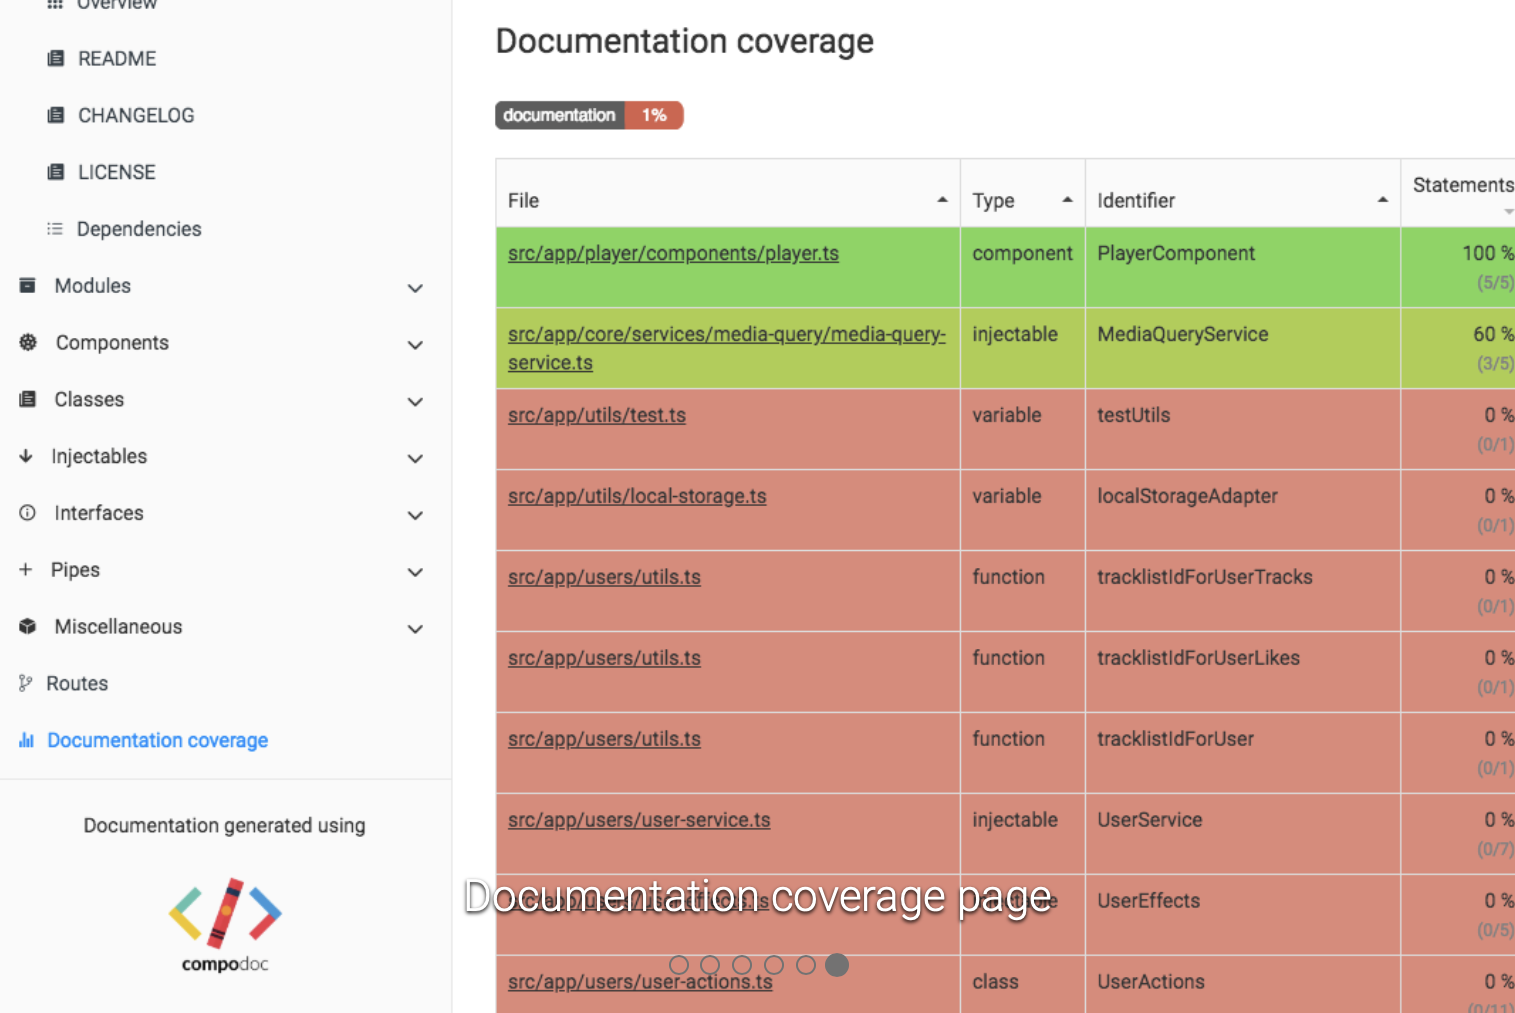
\includegraphics[width = 0.9\linewidth]{img/compodoc.png}

Angular è stato scelto per la realizzazione della WebApp lato front-end, pertanto si è resa necessaria la ricerca di un tool per generare la documentazione relativa a quanto prodotto, necessaria ai fini del progetto.

Abbiamo deciso come gruppo di inserire l'utilizzo di questa tipologia di tool nel nostro {\it{Way of Working}} per la creazione e/o il completamento degli altri documenti richiesti.